
\section{Segunda Questão (9 pts)}

\subsection{Análise Analítica}

\numberwithin{equation}{section}
\numberwithin{figure}{section}

O escoamento de um fluido de viscosidade $\mu$ e massa específica $\rho$,
plenamente desenvolvido em regime permanente, em coordenadas cilíndricas,
é modelado pela equação diferencial

\[ -\frac{1}{\rho} \diff{p}{z} + \frac{\mu}{\rho} \frac{1}{r} \frac{d}{dr} \left(r\diff{u}{r}\right) = 0 \]

\noindent note que podemos cancelar a massa específica $\rho$, obtendo

\begin{equation}\label{eq:modeloQ2}
    \frac{1}{r} \frac{d}{dr} \left(r\diff{u}{r}\right) = \diff{p}{z} \frac{1}{\mu}
\end{equation}

Com um gradiente de pressão constante, temos que a velocidade axial $u$
é uma função de apenas uma variável $r$. Assim, temos as condições de contorno:

\begin{equation}\label{eq:modeloQ2Contorno}
    \begin{cases}
        u(0) = \un{simetria} \logo \diff{u}{r} = 0, \\
        u(R) = 0                                    \\
    \end{cases}
\end{equation}

\noindent onde $R$ é o raio da tubulação por onde o fluido está escoando. Quando
$r = R$ estamos em contato com as paredes da tubulação, que naturalmente têm
velocidade nula. A primeira condição de contorno (simetria) é consequência do sistema de coordenadas
cilíndricas adotado. A Figura \ref*{fig:geometriaQ2} exibe a geometria do problema analisado.

\begin{figure}[h!]
    \caption{Geometria da questão 2.}
    \label{fig:geometriaQ2}
    \centering
    \centerline{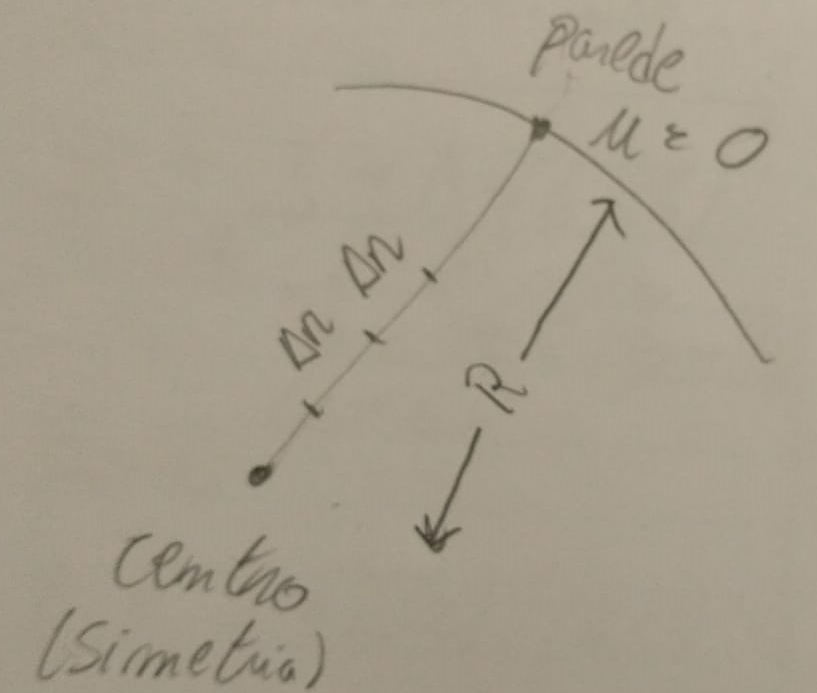
\includegraphics[scale=0.35]{geometriaQ2.png}}
    \par{Fonte: elaboração própria.}
\end{figure}

Note, na Figura \ref*{fig:geometriaQ2}, que estamos analisando o problema em apenas uma dimensão. Como o escoamento
é simétrico em todas as linhas radias do centro à parede, basta analisar o que acontece em uma delas para modelar o 
escoamento inteiro.

Como \eqref{eq:modeloQ2} é uma EDO de primeira ordem, podemos tentar obter uma solução
analítica por integração direta.

\[ \int \frac{d}{dr} \left(r\diff{u}{r}\right) \, dr = \int r \diff{p}{z} \frac{1}{\mu} \, dr \]

\[ r \diff{u}{r} = \frac{r^2}{2} \diff{p}{z} \frac{1}{\mu} + C_1 \]

\[ \int \diff{u}{r} \, dr = \int  \frac{r}{2} \diff{p}{z} \frac{1}{\mu} + \frac{C_1}{r} \, dr \]

\begin{equation}\label{eq:Q2AnaliticGeral}
    u(r) = \frac{r^2}{4} \diff{p}{z} \frac{1}{\mu} + C_1 ln (r) + C_2
\end{equation}

A equação \eqref{eq:Q2AnaliticGeral} é a solução geral para a EDO \eqref{eq:modeloQ2}.
Para que ela atenda às condições de contorno de \eqref{eq:modeloQ2Contorno}, de imediato
temos $C_1 = 0$, pois o logaritmo natural não está definido para $r = 0$,
sendo que fisicamente já sabemos que há uma velocidade no centro da tubulação. Assim,
\eqref{eq:Q2AnaliticGeral} se reduz a

\[ u(r) = \frac{r^2}{4} \diff{p}{z} \frac{1}{\mu} + C_2 \]

A constante $C_2$ pode ser identificada usando a condição de contorno $u(R) = 0$:

\[ 0 = \frac{R^2}{4} \diff{p}{z} \frac{1}{\mu} + C_2 \]

\[ C_2 = - \frac{R^2}{4} \diff{p}{z} \frac{1}{\mu} \]

Assim, a solução analítica do problema é

\[ u(r) = \frac{r^2}{4} \diff{p}{z} \frac{1}{\mu} - \frac{R^2}{4} \diff{p}{z} \frac{1}{\mu}  \]

\begin{equation}\label{eq:Q2Analitic}
    u(r) = \frac{1}{4} \diff{p}{z} \frac{1}{\mu} \left(r^2 - R^2\right)
\end{equation}

No problema temos os seguintes parâmetros:

\begin{itemize}
    \item Raio do tubo: $R=25 \un{mm}$
    \item Viscosidade: $\mu=1.01 \cdot 10^{-3} \un{ kg m$^{-1}$ s$^{-1}$}$
    \item Gradiente de pressão: $\diff{p}{z}=-12.928 \un{N/m}$
    \item Massa específica: $\rho=998 \un{kg m$^{-3}$}$
\end{itemize}

Com esses parâmetros, a Figura \ref*{fig:graficoAnaliticoQ2} mostra o perfil
de velocidade em função da posição radial $r$ dentro da tubulação conforme a solução analítica em
\eqref{eq:Q2Analitic}.

\begin{figure}[h!]
    \caption{Solução analítica da questão 2.}
    \label{fig:graficoAnaliticoQ2}
    \centering
    \centerline{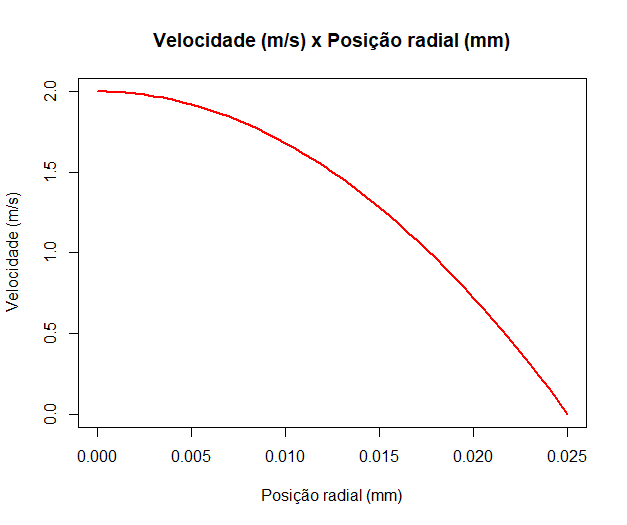
\includegraphics[scale=0.5]{graficoAnaliticoQ2.png}}
    \par{Fonte: elaboração própria.}
\end{figure}

O perfil de velocidade da Figura \ref*{fig:graficoAnaliticoQ2} é condizente com o
esperado fisicamente: a velocidade é máxima no centro do tubo, e zero nas paredes na tubulação,
atendendo também às condições de contorno de \eqref{eq:modeloQ2Contorno}.
Além disso, igual visto durante as aulas da disciplina, temos um perfil parabólico para o
escoamento plenamente desenvolvido na tubulação.

\subsection{Análise Numérica}

Concluída a análise analítica, podemos realizar uma análise numérica do problema. De modo semelhante
ao feito na Questão 1, o primeiro passo é discretizar a equação diferencial \eqref{eq:modeloQ2} via
diferenças finitas.

\[ \frac{d}{dr} \left(r\diff{u}{r}\right) = r \diff{p}{z} \frac{1}{\mu} \]

\noindent aplicando a regra do produto no primeiro membro da equação,

\[ \diff{u}{r} + r \diff[2]{u}{r} = r \diff{p}{z} \frac{1}{\mu} \]

\noindent agora substituimos os diferenciais por diferenças finitas:

\[ \frac{u_{i+1} - u_i}{\Delta r} + r \left(\frac{u_{i+1} - 2u_i + u_{i-1}}{\left(\Delta r\right)^2}\right) = r \diff{p}{z} \frac{1}{\mu} \]

\[ u_{i+1} - u_i + r \left(\frac{u_{i+1} - 2u_i + u_{i-1}}{\Delta r}\right) = (\Delta r) r \diff{p}{z} \frac{1}{\mu} \]

\noindent agrupando as velocidades,

\begin{equation}\label{eq:Q2implicit}
    \begin{split}
        u_{i+1} \left(1 + \frac{r}{\Delta r}\right) + u_i \left(-1 - 2\frac{r}{\Delta r}\right) \\ + u_{i-1} \left(\frac{1}{\Delta r}\right) = (\Delta r) r \diff{p}{z} \frac{1}{\mu}
    \end{split}
\end{equation}

Note que \eqref{eq:Q2implicit} é a forma implícita de diferenças finitas para os nós
internos do domínio. Os termos ligados às velocidades são os coeficientes do sistema linear,
e o segundo membro de \eqref{eq:Q2implicit} tem os coeficientes independentes do sistema linear.

Antes de tentar montar o sistema linear em software, precisamos identificar as equações dos nós do
contorno da geometria. Na parede, temos condição de contorno $u(R) = 0$, logo a equação para $i = R$ é

\begin{equation}\label{eq:Q2implicitBoundary}
    u_i = 0
\end{equation}

Além disso, na linha de centro temos simetria, dada matematicamente por

\[ \diff{u}{r} = 0 \]

Durante a análise analítica, vimos que

\[ \diff{u}{r} = \frac{r}{2} \diff{p}{z} \frac{1}{\mu} + \frac{C_1}{r} \]

\noindent com $C_1 = 0$,

\[ \diff{u}{r} = \frac{r}{2} \diff{p}{z} \frac{1}{\mu} \]

Discretizando a expressão acima, e usando $r = \Delta r / 2$ para analisarmos
o que está acontecendo no nó central, temos

\[ \frac{u_{i+1} - u_i}{\Delta r} = \frac{\Delta r / 2}{2} \diff{p}{z} \frac{1}{\mu} \]

\begin{equation}\label{eq:Q2implicitSimetria}
    u_{i+1} - u_i = \frac{\left(\Delta r\right)^2}{4} \diff{p}{z} \frac{1}{\mu}
\end{equation}

Assim, quando estivermos percorrendo cada $\Delta r$ no domínio, identificamos se ele é um nó interno, nó central ou
nó em contato com as paredes. Em seguida usamos a seguinte metodologia:

\begin{itemize}
    \item Se estamos em um nó interno, calcula os coeficientes através de \eqref{eq:Q2implicit}
    \item Se estamos na parede, calcula os coeficientes através de \eqref{eq:Q2implicitBoundary}
    \item Se estamos no nó central, calcula os coeficientes através de \eqref{eq:Q2implicitSimetria}
\end{itemize}

Uma vez calculados todos os coeficientes, teremos uma matriz de coeficientes $A$ de dimensão $N \times N$, onde
$N = R / \Delta y$, e um vetor de coeficientes independentes $B$ de dimensão $N \times 1$.
O vetor solução $X$, que contém as velocidades $u$ de cada nó, tem dimensão $N \times 1$ e é calculado através da
equação matricial

\begin{equation}\label{eq:Q2sistemalinear}
    X = A^{-1} B
\end{equation}

O pseudocódigo abaixo mostra a ideia principal do software desenvolvido em R que implementa
essa solução numérica. O software completo pode ser visto no ANEXO B.

\begin{algorithmic}
    \State N $\gets$ $R / \Delta y$
    \State A $\gets$ Matriz($N \times N$)
    \State B $\gets$ Vetor($N \times 1$)
    \State $i \gets 0$
    \For{\texttt{cada $\Delta y$ em $R$}}
        \If{$\Delta y$ atual é nó interno}
            \State A[linha $i$] $\gets$ equação \eqref{eq:Q2implicit}
            \State B[$i$] $\gets$ equação \eqref{eq:Q2implicit}
        \EndIf

        \If{$\Delta y$ atual é parede}
            \State A[linha $i$] $\gets$ equação \eqref{eq:Q2implicitBoundary}
            \State B[$i$] $\gets$ equação \eqref{eq:Q2implicitBoundary}
        \EndIf

        \If{$\Delta y$ atual é nó central}
            \State A[linha $i$] $\gets$ equação \eqref{eq:Q2implicitSimetria}
            \State B[$i$] $\gets$ equação \eqref{eq:Q2implicitSimetria}
        \EndIf

        \State $i \gets i + 1$
    \EndFor

    \State X $\gets$ inversa(A) * B

    \Return X
\end{algorithmic}

Ao contrário do problema 1, temos apenas um loop no código. Não temos marcha no tempo uma vez
que o regime de escoamento é permanente. Nesse caso, basta percorrer cada intervalo
$\Delta y$ em $R$, identificar a natureza nesse nó, calcular os coeficientes, jogar nas matrizes
$A$ e $B$ e resolver a equação matricial.

A Figura \ref*{fig:graficoNumericoQ2} mostra uma comparação entre os valores numéricos obtidos no código 
com a solução analítica da Figura \ref*{fig:graficoAnaliticoQ2} para diversas malhas.

\begin{figure*}[h!]
    \caption{Solução numérica (azul) e solução analítica (vermelha) para vários valores de $N$.}
    \label{fig:graficoNumericoQ2}
    \centering
    \centerline{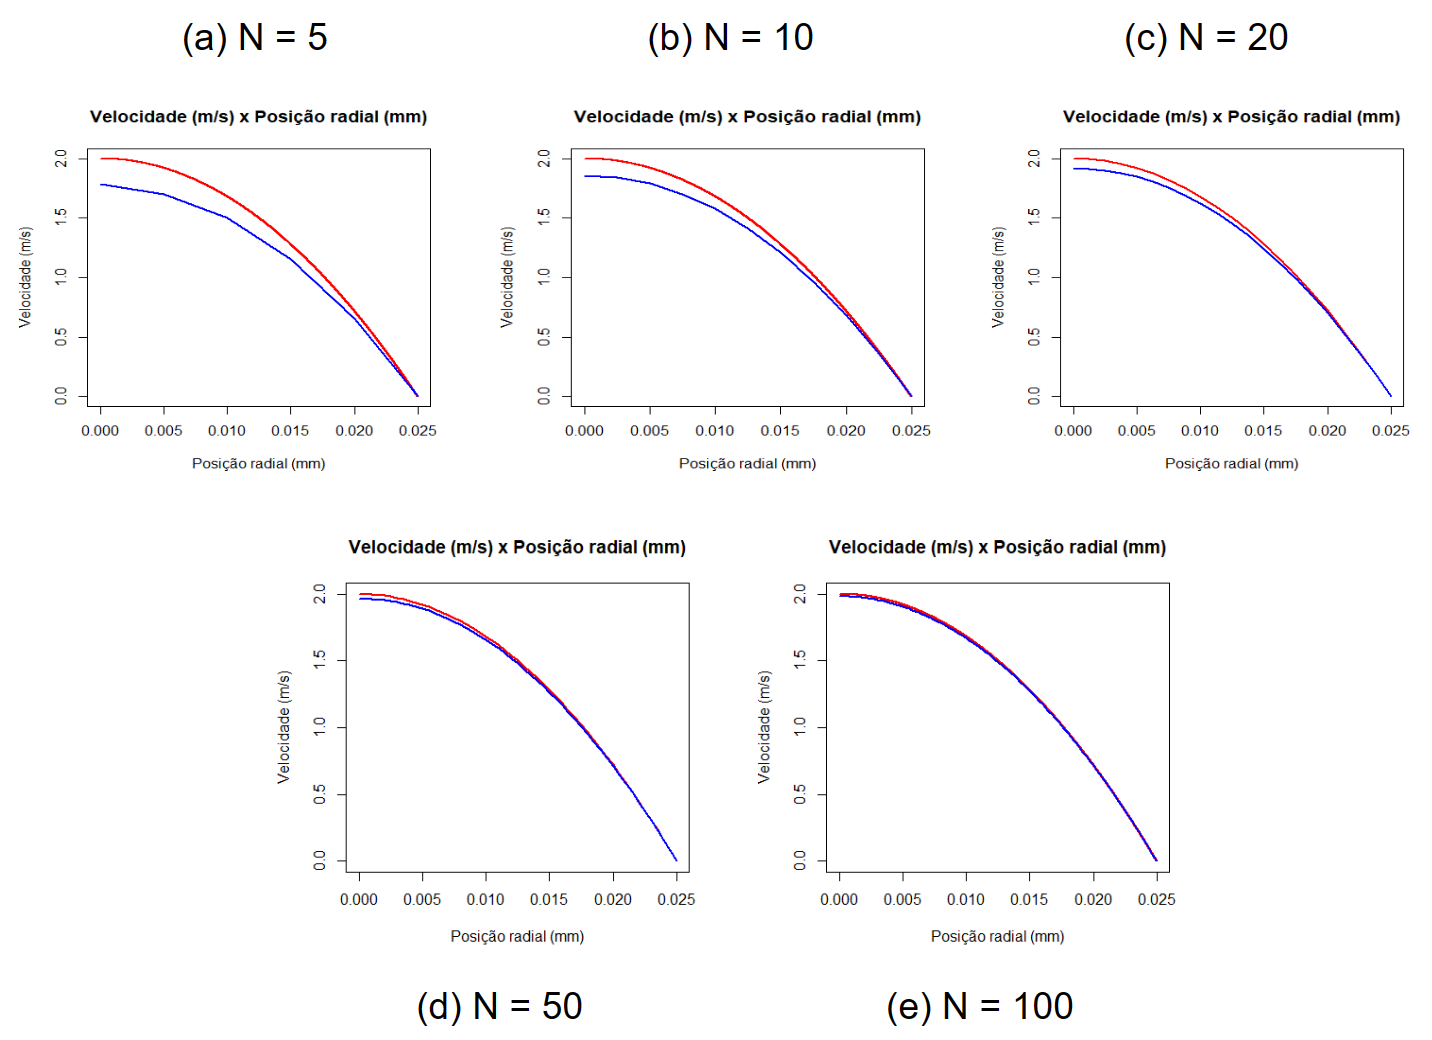
\includegraphics[scale=0.5]{graficoNumericoQ2.png}}
    \par{Fonte: elaboração própria.}
\end{figure*}

Na Figura \ref*{fig:graficoNumericoQ2} (a) temos apenas 5 nós, e a solução obtida está longe da analítica.
Além disso, é possível ver as retas das diferenças finitas na curva azul, uma vez que $N$ é baixo, e 
assim não temos uma curva suave como a analítica. Conforme $N$ aumenta nas Figuras \ref*{fig:graficoNumericoQ2} (b),
(c) e (d), a solução numérica vai ser aproximando da analítica, ficando cada vez mais suave, até ficar
praticamente idêntica à analítica para $N = 100$.

Com base nos gráficos da Figura \ref*{fig:graficoNumericoQ2}, temos que modelo numérico desenvolvido é
satisfatório para $N \geq 50$. Note que usamos o método implícito, e portanto não precisamos nos preocupar com
critérios de estabilidade como na Problema 1. Nesse sentido, não temos restrições teóricas para o valor máximo
de $N$.
Contudo, o uso de $N$ muito elevando aumenta o custo computacional do software, principalmente da matriz de 
coeficientes que possui $N^2$ elementos. Assim, não é necessário, com base nos dados obtidos, 
usar $N$ muito maior que $100$ para esse modelo.